\documentclass[aspectratio=169]{beamer}

% ---------------------------------------------------------------------------
% Pacotes
% ---------------------------------------------------------------------------
\usepackage[utf8]{inputenc}
\usepackage[T1]{fontenc}
\usepackage[portuguese]{babel}
\usepackage{amsmath,amssymb}
\usepackage{tikz}
\usetikzlibrary{arrows.meta, positioning, fit, backgrounds}
\usepackage{booktabs}
\usepackage{array}
\usepackage{xcolor}
\usepackage{graphicx}
\usepackage{pgfplots}
\pgfplotsset{compat=1.17}

% ---------------------------------------------------------------------------
% Tema
% ---------------------------------------------------------------------------
\usetheme{Madrid}
\usecolortheme{whale}
\setbeamertemplate{navigation symbols}{}
\setbeamertemplate{footline}[frame number]

\definecolor{solargold}{RGB}{212,148,0}
\definecolor{magred}{RGB}{178,34,34}
\definecolor{magblue}{RGB}{25,60,140}
\setbeamercolor{title}{fg=solargold}
\setbeamercolor{frametitle}{bg=magblue!90!black,fg=white}
\setbeamercolor{structure}{fg=magblue}

\title[Solar Classifier]{Solar Classifier: Detecção e Classificação\\de Regiões Ativas Solares com YOLOv11}
\subtitle{Da imagem magnética bruta à classificação de Mount Wilson}
\author{Paulo Ricardo Rotband Rangel}
\date{\today}

% ---------------------------------------------------------------------------
\begin{document}

% ---------------------------------------------------------------------------
\begin{frame}
  \titlepage
\end{frame}

\begin{frame}{Sumário}
  \tableofcontents
\end{frame}

% ===========================================================================
\section{Motivação}
% ===========================================================================

\begin{frame}{Por que classificar Regiões Ativas?}
  \begin{itemize}
    \item \textbf{Regiões Ativas (ARs)}: áreas do Sol com forte concentração de campo magnético, visíveis como manchas solares (\emph{sunspots}).
    \item São a origem de \textbf{erupções solares (flares)} e \textbf{ejeções de massa coronal (CMEs)}.
    \item Eventos intensos podem afetar:
    \begin{itemize}
      \item Satélites e comunicações de rádio;
      \item Redes elétricas (tempestades geomagnéticas);
      \item Missões espaciais tripuladas.
    \end{itemize}
    \item \textbf{Ideia central do projeto}: quanto mais complexa a topologia magnética de uma AR, maior a probabilidade de flares fortes.
    \item Objetivo: automatizar a \textbf{detecção} (onde está a AR) e a \textbf{classificação} (quão complexa ela é) usando visão computacional.
  \end{itemize}
\end{frame}

% ===========================================================================
\section{Classificação de Mount Wilson}
% ===========================================================================

\begin{frame}{O que é a Classificação de Mount Wilson?}
  \begin{itemize}
    \item Criada no \textbf{Observatório de Mount Wilson} para descrever a \textbf{complexidade magnética} de uma região ativa.
    \item Baseia-se na distribuição espacial das polaridades magnéticas (positiva/negativa) dentro da mancha.
    \item Quanto mais misturadas e próximas as polaridades opostas estiverem, maior o \textbf{gradiente magnético} e maior a energia disponível para reconexão magnética $\rightarrow$ \textbf{flares}.
    \item É o esquema de classificação usado pelo \textbf{NOAA/SWPC} para previsão de clima espacial até hoje.
  \end{itemize}
\end{frame}

\begin{frame}{As Quatro Classes Usadas no Projeto}
  \begin{table}
    \small
    \begin{tabular}{c l l p{5.2cm}}
      \toprule
      \textbf{Classe} & \textbf{Nome} & \textbf{Padrão} & \textbf{Interpretação física} \\
      \midrule
      0 & Alpha & Unipolar & Uma única polaridade dominante; baixa complexidade. \\
      1 & Beta & Bipolar simples & Duas polaridades bem separadas por uma linha de inversão clara. \\
      2 & Beta-Gamma & Bipolar complexo & Polaridades misturadas/entrelaçadas; linha de inversão irregular. \\
      3 & Beta-Gamma-Delta & Complexidade máxima & Polaridades opostas compartilham a mesma penumbra (\emph{delta spot}); altíssima probabilidade de flares X/M. \\
      \bottomrule
    \end{tabular}
  \end{table}
  \vspace{0.3cm}
  \begin{center}
    \textbf{Alpha $\;\rightarrow\;$ Beta $\;\rightarrow\;$ Beta-Gamma $\;\rightarrow\;$ Beta-Gamma-Delta}\\
    \textcolor{magblue}{baixo risco} \hfill \textcolor{magred}{alto risco de flares}
  \end{center}
\end{frame}

% ===========================================================================
\section{YOLO: Detecção de Objetos}
% ===========================================================================

\begin{frame}{O que é YOLO (You Only Look Once)?}
  \begin{itemize}
    \item Família de redes neurais para \textbf{detecção de objetos em tempo real}.
    \item Diferente de abordagens em duas etapas (ex.: R-CNN, que primeiro propõe regiões e depois classifica), o YOLO faz tudo em \textbf{uma única passada} pela rede.
    \item A imagem é tratada como um problema único de \textbf{regressão}: a rede prevê simultaneamente, para cada região da imagem:
    \begin{itemize}
      \item as coordenadas da \textbf{caixa delimitadora} (bounding box);
      \item a \textbf{confiança} de haver um objeto ali;
      \item a \textbf{classe} do objeto.
    \end{itemize}
    \item Resultado: extremamente rápido, adequado tanto para vídeo em tempo real quanto para varreduras em lote de imagens científicas.
  \end{itemize}
\end{frame}

\begin{frame}{Arquitetura Geral: Backbone $\rightarrow$ Neck $\rightarrow$ Head}
  \begin{center}
  \resizebox{\textwidth}{!}{%
  \begin{tikzpicture}[
      block/.style={rectangle, draw, rounded corners, fill=magblue!10,
                    minimum height=1.6cm, minimum width=3.1cm, align=center, font=\small},
      arr/.style={-Stealth, thick}
    ]
    \node[block] (in) {Imagem de\\entrada};
    \node[block, right=0.7cm of in, fill=solargold!15] (bb) {\textbf{Backbone}\\extrai features\\(bordas, texturas,\\formas)};
    \node[block, right=0.7cm of bb, fill=magred!10] (neck) {\textbf{Neck}\\funde features de\\múltiplas escalas\\(objetos grandes/pequenos)};
    \node[block, right=0.7cm of neck, fill=magblue!10] (head) {\textbf{Head}\\prevê caixas,\\confiança e classe};
    \node[block, right=0.7cm of head, fill=solargold!15] (out) {Detecções\\finais};

    \draw[arr] (in) -- (bb);
    \draw[arr] (bb) -- (neck);
    \draw[arr] (neck) -- (head);
    \draw[arr] (head) -- (out);
  \end{tikzpicture}}
  \end{center}
  \vspace{0.3cm}
  \begin{itemize}
    \small
    \item \textbf{Backbone}: convoluções profundas que resumem a imagem em mapas de características.
    \item \textbf{Neck}: combina mapas de diferentes resoluções (útil pois uma AR pode ocupar poucos ou muitos pixels).
    \item \textbf{Head}: camada final que gera as previsões por região da imagem (\emph{anchor-free} nas versões mais recentes).
  \end{itemize}
\end{frame}

\begin{frame}{Por que YOLOv11?}
  \begin{itemize}
    \item Versão mais recente da família YOLO (Ultralytics), com melhorias sobre YOLOv8:
    \begin{itemize}
      \item Blocos convolucionais mais eficientes (menos parâmetros para a mesma precisão);
      \item Módulos de atenção espacial no \emph{neck}, melhorando a detecção de objetos pequenos;
      \item Detecção \emph{anchor-free}: não depende de caixas-âncora pré-definidas, generalizando melhor para objetos de formato/tamanho variável — como manchas solares.
    \end{itemize}
    \item Disponível em múltiplos tamanhos: \texttt{n, s, m, l, x} — trade-off entre velocidade e acurácia.
    \item \textbf{Configuração padrão do projeto}: \texttt{yolo11m.pt} (\emph{medium}, $\sim$20M parâmetros), pré-treinado no \textbf{COCO}, ajustado (\emph{fine-tuning}) para 4 classes solares.
    \item A execução \texttt{solar\_ar-16} (seção de Resultados) usou \texttt{yolo11n.pt} (\emph{nano}) em CPU, variante mais leve para validar o pipeline mais rapidamente.
  \end{itemize}
\end{frame}

% ===========================================================================
\section{Pipeline do Projeto}
% ===========================================================================

\begin{frame}{Visão Geral do Pipeline de Dados}
  \begin{center}
  \resizebox{\textwidth}{!}{%
  \begin{tikzpicture}[
      block/.style={rectangle, draw, rounded corners, fill=magblue!10,
                    minimum height=1.5cm, minimum width=2.6cm, align=center, font=\small},
      lbl/.style={font=\scriptsize\itshape, magblue},
      arr/.style={-Stealth, thick}
    ]
    \node[block] (jsoc) {JSOC\\(FITS)};
    \node[block, right=1.4cm of jsoc, fill=solargold!15] (local) {Armazenamento\\Local};
    \node[block, right=1.4cm of local, fill=magred!10] (png) {PNG +\\WCS JSON};
    \node[block, right=1.4cm of png, fill=solargold!15] (yl) {Labels\\YOLO (.txt)};
    \node[block, right=1.4cm of yl, fill=magblue!10] (model) {Modelo\\YOLOv11};

    \draw[arr] (jsoc) -- (local) node[midway, above, lbl] {download.py};
    \draw[arr] (local) -- (png) node[midway, above, lbl] {preprocess.py};
    \draw[arr] (png) -- (yl) node[midway, above, lbl] {labels.py};
    \draw[arr] (yl) -- (model) node[midway, above, lbl] {train.py};
  \end{tikzpicture}}
  \end{center}
  \vspace{0.5cm}
  \begin{center}
    \textit{Fluxo linear e modular: dados astronômicos brutos $\rightarrow$ dataset pronto para Deep Learning.}
  \end{center}
\end{frame}

\begin{frame}{Etapa 1 — Aquisição de Dados (\texttt{download.py})}
  \begin{itemize}
    \item Fonte: \textbf{JSOC} (Joint Science Operations Center), série \texttt{hmi.M\_720s} — magnetogramas de linha de visão do instrumento \textbf{HMI/SDO}.
    \item \textbf{Protocolo de exportação em 3 etapas} (via HTTP):
    \begin{enumerate}
      \item \textbf{Request}: solicita a exportação de um intervalo de datas;
      \item \textbf{Polling}: aguarda o JSOC processar a solicitação;
      \item \textbf{Streaming}: baixa os arquivos FITS resultantes.
    \end{enumerate}
    \item \textbf{Estratégia de implementação}:
    \begin{itemize}
      \item Assíncrona, usando \texttt{aiohttp};
      \item Grandes períodos são divididos em blocos de \textbf{90 dias} para evitar timeouts no servidor.
    \end{itemize}
  \end{itemize}
\end{frame}

\begin{frame}{Etapa 2 — Pré-processamento (\texttt{preprocess.py})}
  Arquivos FITS não podem ser lidos diretamente por redes neurais — esta etapa converte física em imagem.
  \begin{itemize}
    \item \textbf{Correção de orientação}: verifica e corrige o ângulo \texttt{CROTA2}, garantindo Norte solar sempre para cima.
    \item \textbf{Normalização magnética}:
    \begin{itemize}
      \item Campo magnético (Gauss) clipado em $\pm 1000$ G;
      \item Mapeamento linear para \texttt{uint8 [0, 255]}: Sol calmo (0 G) $\rightarrow$ cinza médio ($\approx 127$).
    \end{itemize}
    \item \textbf{Redimensionamento}: imagens levadas a $1024 \times 1024$ px com interpolação de \textbf{Lanczos}, preservando manchas pequenas.
    \item \textbf{Sidecar WCS} (\emph{World Coordinate System}): arquivo \texttt{.json} com parâmetros de escala/referência — necessário para converter coordenadas do HEK (arcsegundos) em pixels da imagem redimensionada.
  \end{itemize}
\end{frame}

\begin{frame}{Detalhe Técnico: Por que Interpolação de Lanczos?}
  \begin{itemize}
    \item As imagens nativas do HMI têm $4096\times4096$ px ($\approx 0{,}504''$/pixel) — o redimensionamento para $1024\times1024$ é um \textbf{downsampling de $4\times$}.
    \item Métodos simples (\emph{nearest-neighbor}, bilinear) fazem uma média local ingênua: borram ou causam \emph{aliasing} em detalhes pequenos — exatamente o problema, pois manchas isoladas e a \textbf{linha de inversão de polaridade} de um \emph{delta-spot} podem ocupar poucos pixels.
    \item \textbf{Lanczos} usa um kernel de \emph{sinc} janelado:
    $$L(x) = \begin{cases} \text{sinc}(x)\,\text{sinc}\!\left(\dfrac{x}{a}\right), & |x| < a \\[4pt] 0, & \text{caso contrário} \end{cases} \qquad \text{sinc}(x) = \dfrac{\sin(\pi x)}{\pi x}$$
    com $a=3$ (Lanczos-3, padrão do Pillow \texttt{Image.LANCZOS}).
    \item \textbf{Trade-off}: é mais caro computacionalmente e pode gerar leve \emph{ringing} (overshoot) em bordas de altíssimo contraste — aceitável aqui, pois preservar a morfologia da mancha importa mais do que suavidade visual.
    \item Prática comum em processamento de imagens astronômicas (ex.: \texttt{reproject}, \texttt{astropy}) por preservar melhor conteúdo de alta frequência do que bicúbica/bilinear.
  \end{itemize}
\end{frame}

\begin{frame}{Exemplo Real: Magnetograma Pré-processado}
  \begin{center}
    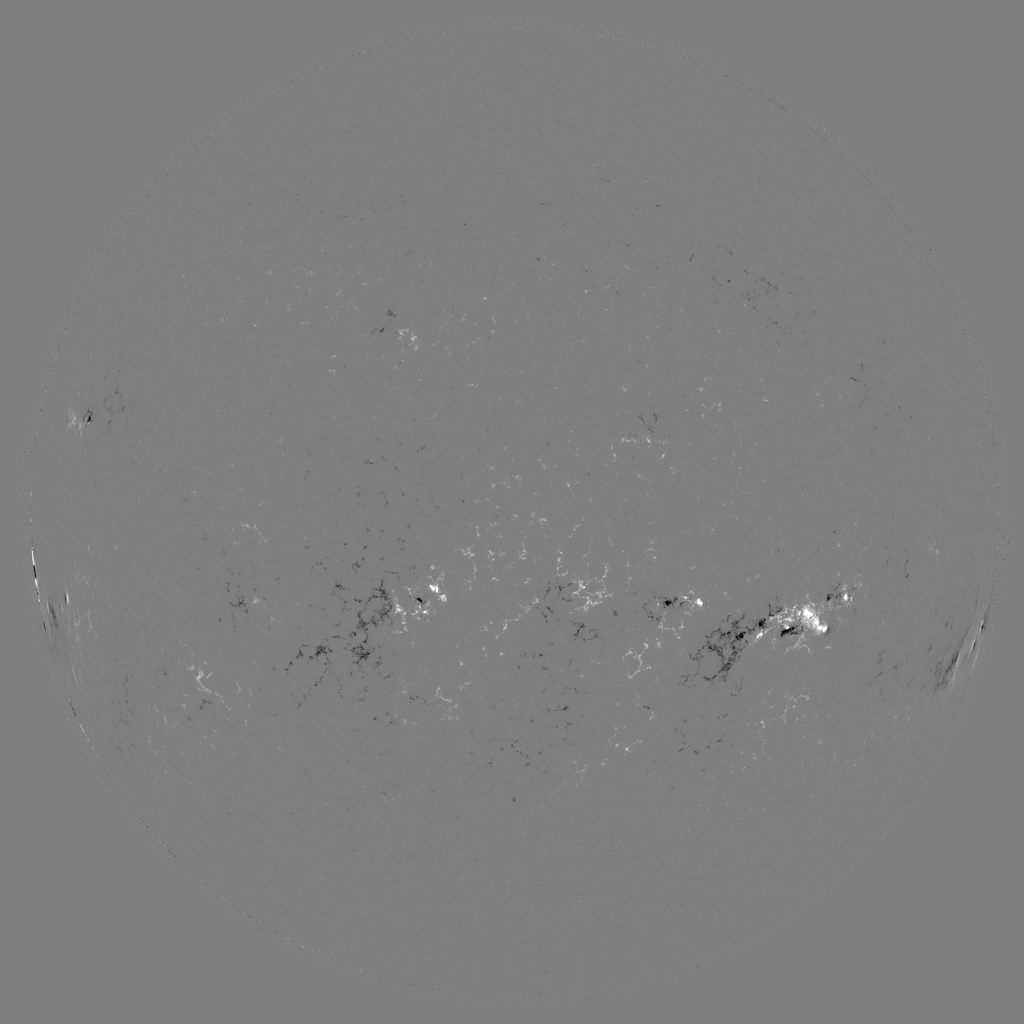
\includegraphics[height=0.68\textheight]{figs/hmi.M_720s.300522.magnetogram.png}
  \end{center}
  \begin{center}
    \footnotesize Magnetograma HMI real do dataset do projeto, após correção de \texttt{CROTA2},\\
    normalização $\pm 1000$~G $\to$ \texttt{uint8} e redimensionamento para $1024\times1024$~px.\\
    Cinza médio = Sol calmo; regiões claras/escuras = polaridades magnéticas opostas.
  \end{center}
\end{frame}

\begin{frame}{Exemplo Real: Labels (Ground Truth) sobre o Magnetograma}
  \begin{center}
    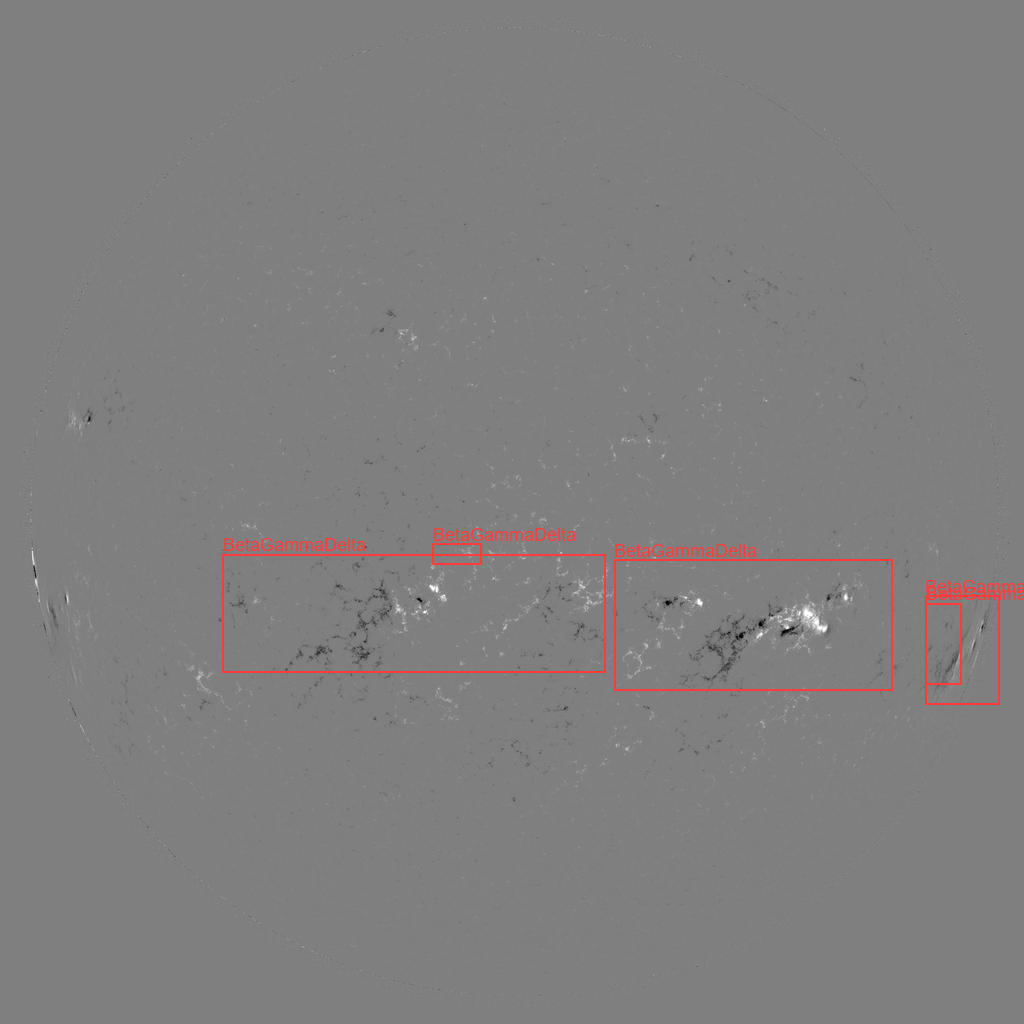
\includegraphics[height=0.65\textheight]{figs/hmi.M_720s.300522.magnetogram_overlay.png}
  \end{center}
  \begin{center}
    \footnotesize Mesma imagem com as caixas YOLO reais do dataset, geradas a partir dos eventos do HEK\\
    (\texttt{src/labels.py}) e sobrepostas via \texttt{src/debug\_overlay.py} para checagem visual da geometria.
  \end{center}
\end{frame}

\begin{frame}{Etapa 3 — Geração de Labels (\texttt{labels.py})}
  As \emph{ground truths} vêm do \textbf{HEK} (Heliophysics Event Knowledgebase).
  \begin{itemize}
    \item \textbf{Estratégia de consulta}: uma query HTTP \textbf{por dia} (não por imagem), eventos armazenados em cache e associados às imagens dentro de uma janela de $\pm 30$ minutos.
    \item \textbf{Geometria da bounding box} — ordem de prioridade:
    \begin{enumerate}
      \item \textbf{SHARP}: fornece a extensão real do \emph{patch} magnético (melhor fonte);
      \item \textbf{SPoCA}: fallback via proximidade espacial;
      \item \textbf{Estimativa por área}: último recurso, baseada na área da região em \textbf{MSH} (\emph{Millionths of Solar Hemisphere}).
    \end{enumerate}
    \item Classes finais mapeadas via \texttt{MTWILSON\_MAP}: \texttt{alpha $\to$ 0, beta $\to$ 1, betagamma/gamma/betadelta $\to$ 2, betagammadelta $\to$ 3}.
  \end{itemize}
\end{frame}

\begin{frame}{Detalhe Técnico: SHARP (fonte primária da bbox)}
  \textbf{SHARP} — \emph{Space-weather HMI Active Region Patches} (Bobra et al. 2014).
  \begin{itemize}
    \item Módulo automático do pipeline HMI que \textbf{detecta e rastreia} concentrações de campo magnético vetorial ao longo de todo o trânsito da AR pelo disco ($\sim$2 semanas), a cada 12 minutos.
    \item Gera dois tipos de recorte por região: \texttt{CCD} (pixel nativo) e \texttt{CEA} (projeção \emph{Cylindrical Equal-Area}, que remove o efeito de escorço perto do limbo solar).
    \item Os metadados trazem diretamente a \textbf{extensão heliográfica real} do \emph{patch} rastreado (não uma estimativa) — por isso é a fonte prioritária de bounding box no projeto.
    \item Cada SHARP carrega o número NOAA da AR, usado para casar com os eventos de classificação Mount Wilson do HEK.
  \end{itemize}
\end{frame}

\begin{frame}{Detalhe Técnico: SPoCA (fallback espacial)}
  \textbf{SPoCA} — \emph{Spatial Possibilistic Clustering Algorithm} (Verbeeck et al. 2013).
  \begin{itemize}
    \item Algoritmo de \textbf{segmentação não supervisionada}, originalmente criado para detectar Regiões Ativas e Buracos Coronais em imagens EUV (SDO/AIA), também usado para alimentar o HEK com posições de AR.
    \item Baseado em \emph{possibilistic c-means} — uma variante \emph{fuzzy} do k-means: cada pixel recebe um \textbf{grau de pertencimento} a um cluster, em vez de um limiar rígido; mais adequado a bordas difusas de estruturas solares.
    \item \textbf{Uso no projeto}: quando não há SHARP correspondente (ex.: AR ainda sem número NOAA, ou lacuna na cobertura), usa-se a detecção SPoCA mais próxima espacialmente — dá a \emph{posição}, mas não necessariamente a geometria exata da bbox.
  \end{itemize}
\end{frame}

\begin{frame}{Etapa 4 — Treinamento (\texttt{train.py})}
  \begin{itemize}
    \item Arquitetura: \textbf{YOLOv11m} (medium), com \textbf{transfer learning} a partir de pesos pré-treinados no \textbf{COCO}.
    \item O \emph{backbone} já sabe detectar bordas/texturas/blobs genéricos — a rede só precisa adaptar a \emph{head} para as 4 classes solares.
    \item \textbf{Otimização}:
    \begin{itemize}
      \item \emph{Cosine Learning Rate Schedule} (\texttt{cos\_lr=True}) — decaimento suave da taxa de aprendizado;
      \item \emph{Early stopping} (\texttt{patience=20}) — evita overfitting em datasets solares pequenos.
    \end{itemize}
    \item \textbf{Hardware}: suporte a \textbf{CUDA} (Nvidia) e \textbf{DirectML} (AMD GPU, via \texttt{torch-directml}), com fallback para CPU multi-thread.
  \end{itemize}
\end{frame}

\begin{frame}{Restrições Físicas de Augmentation}
  Magnetogramas não são fotos comuns — augmentations padrão podem gerar dados \textbf{fisicamente impossíveis}.
  \begin{itemize}
    \item \texttt{fliplr = 0} (sem espelhamento horizontal):
    \begin{itemize}
      \small \item Inverteria a orientação Leste-Oeste e a \textbf{Lei de Hale} (polaridade líder/seguidora por hemisfério).
    \end{itemize}
    \item \texttt{flipud = 0} (sem espelhamento vertical):
    \begin{itemize}
      \small \item Inverteria Norte/Sul e a \textbf{Lei de Joy}, que dita a inclinação estatística dos grupos bipolares em relação ao equador.
    \end{itemize}
    \item \texttt{hsv\_h = 0}, \texttt{hsv\_s = 0} (sem matiz/saturação):
    \begin{itemize}
      \small \item Dados são grayscale de 1 canal — matiz e saturação não têm significado físico.
    \end{itemize}
    \item \texttt{hsv\_v = 0.02}: leve jitter de brilho mantido, simulando variações de calibração do HMI sem distorcer a polaridade.
  \end{itemize}
\end{frame}

\begin{frame}{Detalhe Técnico: Lei de Hale (Polaridade Magnética)}
  \begin{itemize}
    \item Descrita por Hale, Ellerman, Nicholson \& Joy (1919) — o mesmo artigo que origina a classificação de Mount Wilson.
    \item Em grupos bipolares, a mancha \textbf{líder} (mais a oeste, no sentido da rotação) tem sempre a \textbf{mesma polaridade} em todo um hemisfério solar durante um dado ciclo de 11 anos; o hemisfério oposto tem polaridade líder invertida.
    \item Esse padrão \textbf{se inverte} a cada novo ciclo de 11 anos — por isso o ciclo magnético completo do Sol (\emph{ciclo de Hale}) dura $\approx 22$ anos.
    \item \textbf{Consequência para o augmentation} (\texttt{fliplr=0}): espelhar horizontalmente troca a mancha líder pela seguidora, o que equivale a simular o hemisfério errado ou a metade errada do ciclo solar — uma combinação que praticamente nunca ocorre na natureza. Treinar com esses dados ensinaria ao modelo um padrão de polaridade fisicamente impossível.
  \end{itemize}
\end{frame}

\begin{frame}{Detalhe Técnico: Lei de Joy (Inclinação dos Grupos)}
  \begin{itemize}
    \item Relatada por Alfred Joy no mesmo artigo de 1919: grupos bipolares não são alinhados perfeitamente Leste-Oeste — são \textbf{inclinados}, com a mancha líder ligeiramente mais próxima do equador que a seguidora.
    \item O ângulo de inclinação \textbf{cresce com a latitude} heliográfica da região (tendência estatística, com dispersão considerável região a região).
    \item \textbf{Origem física} (modelo de Babcock--Leighton): a força de \textbf{Coriolis} atua sobre o tubo de fluxo magnético torcido enquanto ele ascende por flutuação através da zona de convecção, torcendo o par de manchas nesse sentido preferencial.
    \item \textbf{Consequência para o augmentation} (\texttt{flipud=0}): espelhar verticalmente inverte Norte/Sul e, com isso, o sinal dessa inclinação estatística — ensinaria ao modelo uma relação inclinação-latitude que viola a física do dínamo solar real.
  \end{itemize}
\end{frame}

% ===========================================================================
\section{Avaliação}
% ===========================================================================

\begin{frame}{Métricas de Avaliação}
  \begin{itemize}
    \item \textbf{mAP50} (\emph{mean Average Precision} @ IoU 0.50):
    \begin{itemize}
      \small \item Padrão em detecção de objetos solares/sensoriamento remoto; considera uma detecção correta se a sobreposição (IoU) com a caixa real for $\geq 50\%$.
    \end{itemize}
    \item \textbf{mAP50-95}:
    \begin{itemize}
      \small \item Média sobre limiares de IoU de 0.50 a 0.95 (passo 0.05) — métrica estilo COCO, mais rigorosa quanto à precisão de localização.
    \end{itemize}
    \item \textbf{IoU} (\emph{Intersection over Union}):
    $$\text{IoU} = \frac{\text{Área de Interseção}}{\text{Área de União}}$$
    entre a caixa prevista e a caixa real (\emph{ground truth}).
  \end{itemize}
\end{frame}

\begin{frame}{Tabela de Referências Técnicas}
  \begin{table}
    \small
    \begin{tabular}{p{2.6cm} p{3.4cm} p{5cm}}
      \toprule
      \textbf{Conceito} & \textbf{Referência no código} & \textbf{Significado} \\
      \midrule
      Séries HMI & \texttt{src/download.py} & Dados de magnetometria do SDO. \\
      WCS Projection & \texttt{src/preprocess.py} $\to$ sidecar & Coordenadas esféricas $\to$ pixels. \\
      Mount Wilson & \texttt{src/labels.py} $\to$ \texttt{MTWILSON\_MAP} & Escala de complexidade magnética. \\
      Lei de Joy & \texttt{src/train.py} $\to$ \texttt{flipud=0} & Regra física da inclinação das ARs. \\
      mAP50 & \texttt{src/train.py} $\to$ \texttt{evaluate()} & Métrica de precisão de detecção. \\
      \bottomrule
    \end{tabular}
  \end{table}
\end{frame}

% ===========================================================================
\section{Resultados (run \texttt{solar\_ar-16})}
% ===========================================================================

\begin{frame}{Configuração da Execução \texttt{solar\_ar-16}}
  \begin{table}
    \small
    \begin{tabular}{l l}
      \toprule
      \textbf{Parâmetro} & \textbf{Valor} \\
      \midrule
      Modelo & \texttt{yolo11n.pt} (nano, COCO pré-treinado) \\
      Dispositivo & CPU (sem AMP) \\
      Imagem & $1024 \times 1024$ px \\
      Batch & 8 \\
      Épocas configuradas & 100 (\texttt{patience=20}, \texttt{cos\_lr=True}) \\
      Épocas efetivamente rodadas & 24 \\
      Augmentation & \texttt{fliplr=0}, \texttt{flipud=0}, \texttt{hsv\_h=hsv\_s=0} \\
      \bottomrule
    \end{tabular}
  \end{table}
  \vspace{0.2cm}
  \small \textit{Fonte: \texttt{runs/solar\_ar-16/args.yaml} e \texttt{results.csv}.}
\end{frame}

\begin{frame}{Distribuição Real das Classes no Treino}
  \begin{center}
    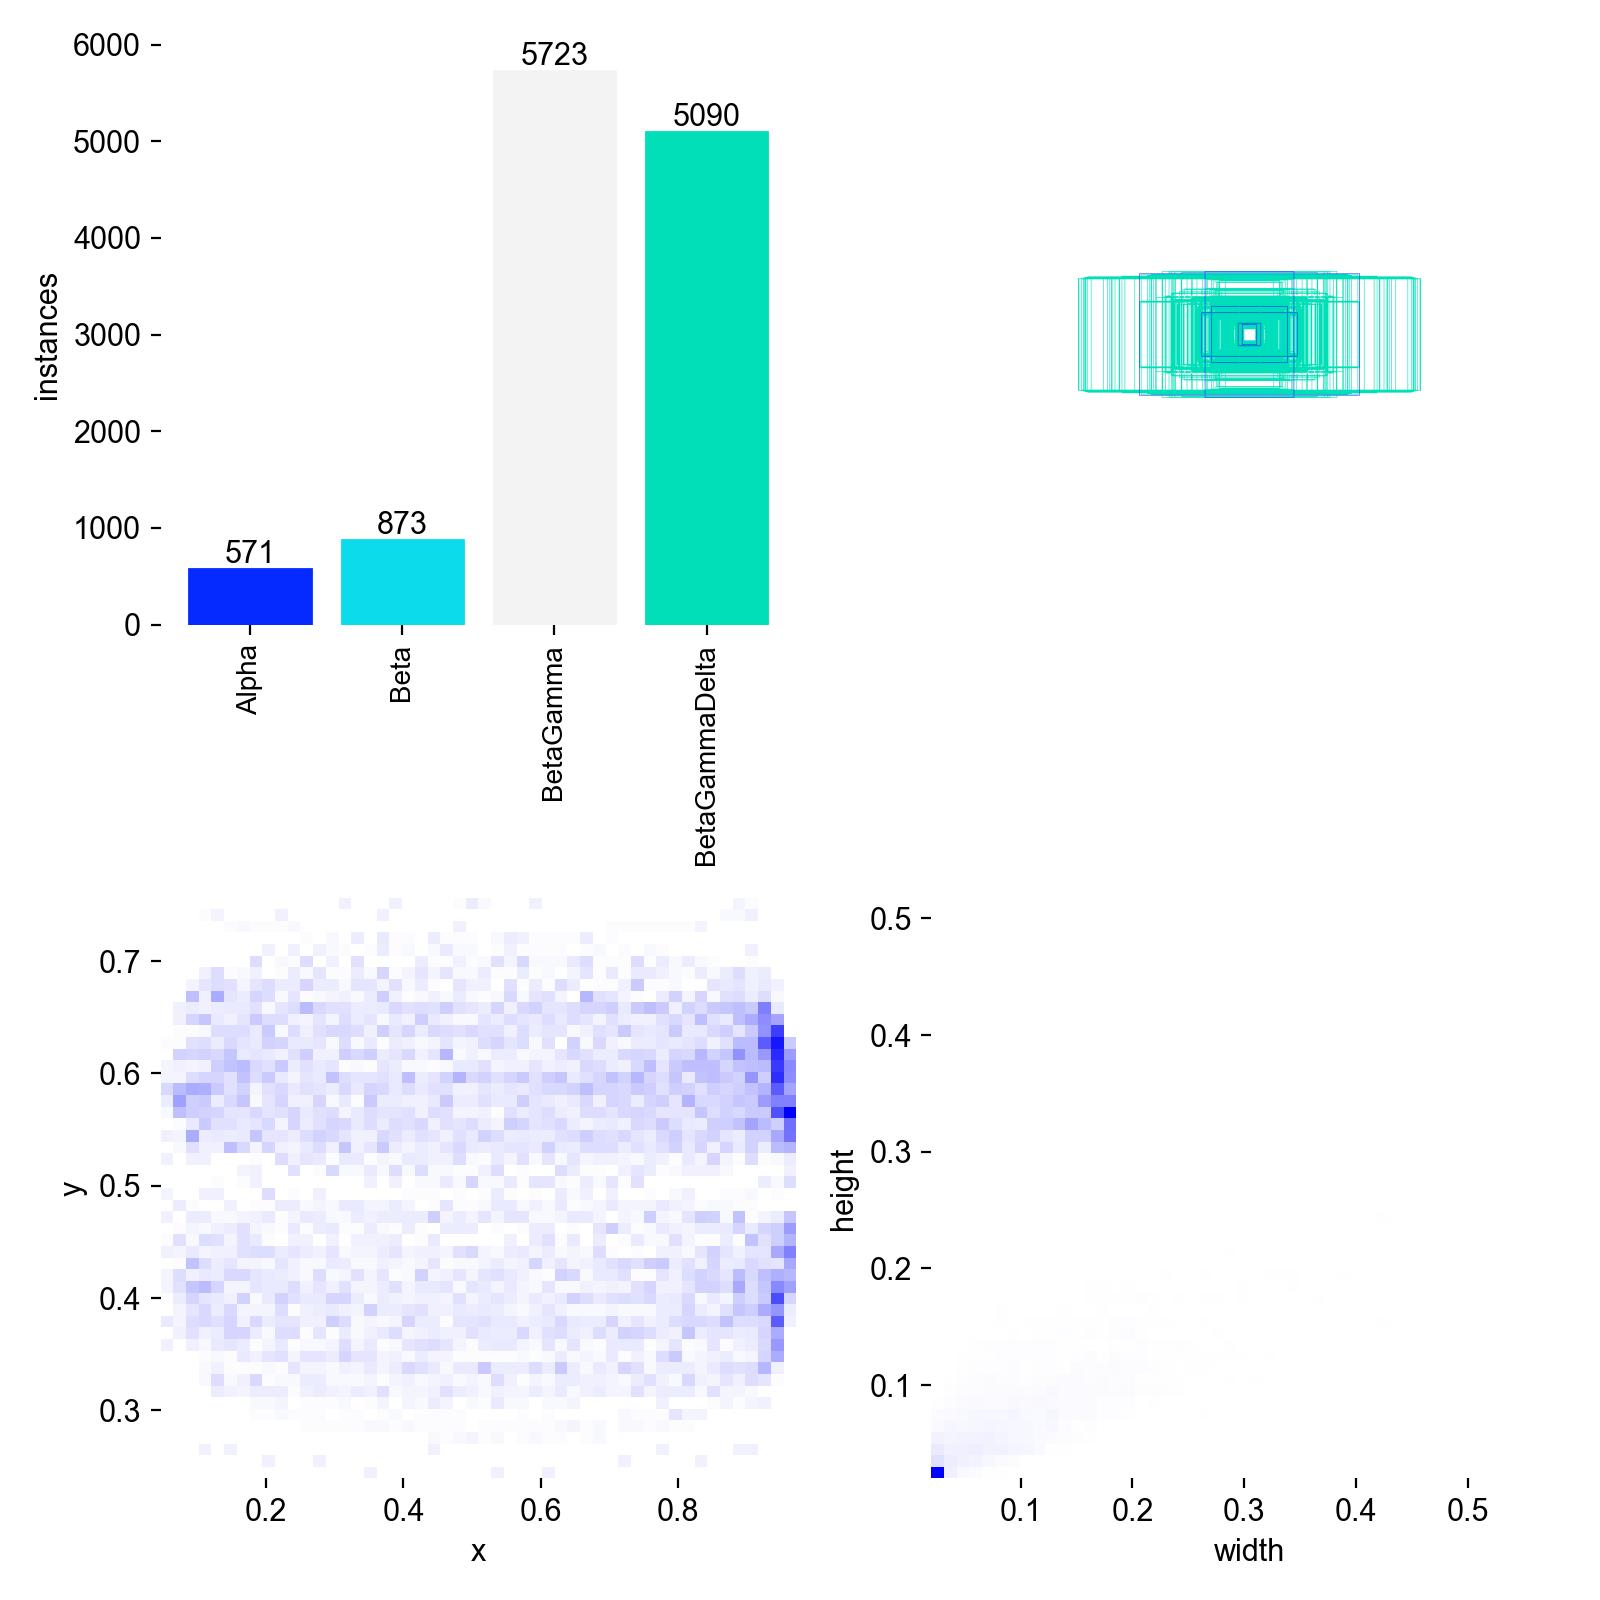
\includegraphics[height=0.72\textheight]{figs/solar_ar-16_labels.jpg}
  \end{center}
  \begin{center}
    \footnotesize Instâncias por classe: Alpha 571 · Beta 873 · Beta-Gamma 5723 · Beta-Gamma-Delta 5090.\\
    Forte \textbf{desbalanceamento} a favor das classes mais complexas — ponto de atenção para trabalhos futuros.
  \end{center}
\end{frame}

\begin{frame}{Evolução do mAP ao Longo do Treino}
  \begin{center}
  \begin{tikzpicture}
    \begin{axis}[
        width=0.95\textwidth, height=6cm,
        xlabel={Época}, ylabel={mAP},
        legend pos=north west, legend style={font=\scriptsize},
        ymin=0, ymax=0.22,
        grid=major, grid style={gray!20},
        label style={font=\small}, tick label style={font=\scriptsize}
      ]
      \addplot[magblue, thick, mark=*, mark size=1pt] coordinates {
        (1,0.13415)(2,0.12135)(3,0.01031)(4,0.09945)(5,0.17503)(6,0.13667)
        (7,0.13631)(8,0.02820)(9,0.10522)(10,0.00143)(11,0.00266)(12,0.18529)
        (13,0.00157)(14,0.04487)(15,0.00194)(16,0.01886)(17,0.02588)(18,0.19906)
        (19,0.14309)(20,0.00472)(21,0.00049)(22,0.12799)(23,0.09705)(24,0.00136)
      };
      \addlegendentry{mAP50}
      \addplot[magred, thick, mark=square*, mark size=1pt] coordinates {
        (1,0.06632)(2,0.06167)(3,0.00372)(4,0.03060)(5,0.09334)(6,0.04752)
        (7,0.05661)(8,0.01455)(9,0.04790)(10,0.00024)(11,0.00035)(12,0.10502)
        (13,0.00028)(14,0.01250)(15,0.00040)(16,0.00670)(17,0.00801)(18,0.11521)
        (19,0.07921)(20,0.00067)(21,0.00006)(22,0.06085)(23,0.05453)(24,0.00027)
      };
      \addlegendentry{mAP50-95}
    \end{axis}
  \end{tikzpicture}
  \end{center}
  \footnotesize \textit{Fonte: \texttt{runs/solar\_ar-16/results.csv}. Alta variância entre épocas — esperado em dataset pequeno.}
\end{frame}

\begin{frame}{Perda de Treino vs. Validação}
  \begin{center}
  \begin{tikzpicture}
    \begin{axis}[
        width=0.95\textwidth, height=6cm,
        xlabel={Época}, ylabel={Loss total (box+cls+dfl)},
        legend pos=north east, legend style={font=\scriptsize},
        ymin=0, ymax=14,
        grid=major, grid style={gray!20},
        label style={font=\small}, tick label style={font=\scriptsize}
      ]
      \addplot[magblue, thick, mark=*, mark size=1pt] coordinates {
        (1,7.30458)(2,6.16239)(3,5.85624)(4,5.70920)(5,5.47020)(6,5.36460)
        (7,5.22605)(8,5.14455)(9,5.09700)(10,5.01863)(11,4.96143)(12,4.90692)
        (13,4.79791)(14,4.78926)(15,4.69545)(16,4.62057)(17,4.56800)(18,4.49322)
        (19,4.39783)(20,4.39415)(21,4.30832)(22,4.22655)(23,4.21659)(24,4.19921)
      };
      \addlegendentry{Treino}
      \addplot[magred, thick, mark=square*, mark size=1pt] coordinates {
        (1,6.97363)(2,7.35183)(3,9.61494)(4,7.46211)(5,5.68102)(6,7.07795)
        (7,6.78534)(8,9.24868)(9,6.97611)(10,12.03178)(11,13.28812)(12,5.69450)
        (13,10.87635)(14,9.58673)(15,11.17278)(16,10.22996)(17,9.76405)(18,5.15680)
        (19,5.53204)(20,11.71166)(21,11.68848)(22,6.24486)(23,6.64406)(24,11.97671)
      };
      \addlegendentry{Validação}
    \end{axis}
  \end{tikzpicture}
  \end{center}
  \footnotesize \textit{Fonte: \texttt{runs/solar\_ar-16/results.csv} (soma de \texttt{box\_loss+cls\_loss+dfl\_loss}).\\
  A perda de treino cai de forma suave e monotônica; a de validação oscila fortemente entre épocas —\\
  sinal de \textbf{overfitting} e de um conjunto de validação pequeno demais para estabilizar a métrica.}
\end{frame}

\begin{frame}{Melhor Checkpoint (\texttt{best.pt})}
  \begin{table}
    \begin{tabular}{l c}
      \toprule
      \textbf{Métrica (época 18)} & \textbf{Valor} \\
      \midrule
      Precision & 0.251 \\
      Recall & 0.398 \\
      mAP50 & 0.199 \\
      mAP50-95 & 0.115 \\
      \bottomrule
    \end{tabular}
  \end{table}
  \vspace{0.3cm}
  \textbf{Leitura honesta dos resultados:}
  \begin{itemize}
    \small
    \item Modelo \texttt{nano} em CPU, com poucas épocas — resultado é uma \textbf{prova de conceito}, não um modelo de produção.
    \item Grande variância de métricas entre épocas sugere dataset ainda pequeno para o modelo estabilizar.
    \item Desbalanceamento de classes (slide anterior) provavelmente penaliza Alpha e Beta na precisão.
    \item Próximo passo natural: mais dados, \texttt{yolo11m}/\texttt{l} em GPU, e re-balanceamento de classes.
  \end{itemize}
\end{frame}

% ===========================================================================
\section{Referências}
% ===========================================================================

\begin{frame}{Referências — Dados e Instrumentação}
  \small
  \begin{itemize}
    \item SDO/HMI — Instrument overview:\\
      \href{https://sdo.gsfc.nasa.gov/mission/instruments/hmi.php}{\texttt{sdo.gsfc.nasa.gov/mission/instruments/hmi.php}}
    \item JSOC — Joint Science Operations Center (acesso aos dados HMI):\\
      \href{http://jsoc.stanford.edu}{\texttt{jsoc.stanford.edu}}
    \item HEK — Heliophysics Event Knowledgebase:\\
      \href{https://www.lmsal.com/hek/}{\texttt{lmsal.com/hek}}\\
      \footnotesize Hurlburt, N. et al. (2012). \textit{Heliophysics Event Knowledgebase for the Solar Dynamics Observatory (SDO) and Beyond}. Solar Physics, 275, 67–78.
    \item SHARP — Space-weather HMI Active Region Patches:\\
      \footnotesize Bobra, M. G. et al. (2014). \textit{The Helioseismic and Magnetic Imager (HMI) Vector Magnetic Field Pipeline: SHARPs}. Solar Physics, 289, 3549–3578.
  \end{itemize}
\end{frame}

\begin{frame}{Referências — Classificação Solar}
  \small
  \begin{itemize}
    \item Classificação magnética de Mount Wilson (origem):\\
      \footnotesize Hale, G. E., Ellerman, F., Nicholson, S. B., \& Joy, A. H. (1919). \textit{The Magnetic Polarity of Sun-Spots}. The Astrophysical Journal, 49, 153.
    \item \normalsize Lei de Joy / Lei de Hale — inclinação e polaridade de grupos bipolares:\\
      \footnotesize van Driel-Gesztelyi, L. \& Green, L. M. (2015). \textit{Evolution of Active Regions}. Living Reviews in Solar Physics, 12, 1.
    \item \normalsize Esquema estendido (McIntosh), usado operacionalmente junto ao Mount Wilson:\\
      \footnotesize McIntosh, P. S. (1990). \textit{The classification of sunspot groups}. Solar Physics, 125, 251–267.
    \item \normalsize NOAA / Space Weather Prediction Center (previsão operacional de clima espacial):\\
      \href{https://www.swpc.noaa.gov/}{\texttt{swpc.noaa.gov}}
  \end{itemize}
\end{frame}

\begin{frame}{Referências — YOLO}
  \small
  \begin{itemize}
    \item Artigo original do YOLO:\\
      \footnotesize Redmon, J., Divvala, S., Girshick, R., \& Farhadi, A. (2016). \textit{You Only Look Once: Unified, Real-Time Object Detection}. CVPR 2016. \href{https://arxiv.org/abs/1506.02640}{\texttt{arxiv.org/abs/1506.02640}}
    \item \normalsize Documentação oficial YOLOv11 (Ultralytics):\\
      \href{https://docs.ultralytics.com/models/yolo11/}{\texttt{docs.ultralytics.com/models/yolo11}}
    \item \normalsize Código-fonte Ultralytics:\\
      \href{https://github.com/ultralytics/ultralytics}{\texttt{github.com/ultralytics/ultralytics}}
    \item \normalsize Métricas de detecção (mAP, IoU) — protocolo COCO:\\
      \href{https://cocodataset.org/\#detection-eval}{\texttt{cocodataset.org/\#detection-eval}}
  \end{itemize}
\end{frame}

% ===========================================================================
\section{Conclusão}
% ===========================================================================

\begin{frame}{Conclusão}
  \begin{itemize}
    \item Pipeline completo e reprodutível: \textbf{JSOC $\to$ FITS $\to$ PNG/WCS $\to$ Labels YOLO $\to$ Modelo treinado}.
    \item Combina \textbf{visão computacional moderna} (YOLOv11) com \textbf{restrições físicas do domínio} (Lei de Joy, Lei de Hale, orientação solar).
    \item Classificação automática segundo o esquema de \textbf{Mount Wilson}, usado operacionalmente pelo NOAA para previsão de clima espacial.
    \item Resultado inicial (\texttt{solar\_ar-16}, YOLOv11n/CPU): mAP50 $\approx 0.20$ — prova de conceito do pipeline ponta a ponta, não um modelo final.
    \item Próximos passos: mais dados históricos, modelos maiores (m/l) em GPU, e correção do desbalanceamento de classes.
  \end{itemize}
  \vspace{0.5cm}
  \begin{center}
    \Large \textbf{Perguntas?}
  \end{center}
\end{frame}

\end{document}
